\documentclass[a4paper,ngerman]{tui-algo-seminar}
\usepackage{graphicx}
\usepackage{algorithm2e}
\usepackage{booktabs}
\usepackage{tikz}
\usepackage{hyperref}
\usepackage{float}
\usepackage{listings}
\usepackage{totpages}  % Paket für die Gesamtseitenzahl
\setlength{\footskip}{13.0pt} % keine Ahnung ^^

\usepackage[utf8]{inputenc} % Verwenden Sie utf8 für UTF-8 Zeichencodierung

\newcommand{\inhalt}{8. Gerd Fornahl Turnier 2024}
\seminar{\inhalt}
\semester{\today}
\title{\inhalt}
\author{Erik Skopp}

\usepackage{fancyhdr}  % Für individuelle Kopf- und Fußzeilen
\nolinenumbers

% Definieren des Seitenstils
\pagestyle{fancy}
\fancyhf{}  % Vorherige Kopf- und Fußzeilen-Einstellungen löschen
%\fancyfoot[Rf]{\thepage ~von \zpageref{LastPage}}  % Gesamtseitenzahl

\begin{document}

\maketitle
\thispagestyle{plain} % Seitenzahl auf Seite 1 anzeigen
\begin{abstract}
Bericht: \inhalt.\\
Das 
\end{abstract}

\tableofcontents 
\clearpage
\section{Bericht}
Hier können Sie eine Einführung oder den Haupttext Ihres Berichts einfügen.

\section{Tabellen}

\subsection{Startrangliste}
\begin{table}[h]
\centering
\caption{Teilnehmerliste: Sortiert nach Spielernummer}
\begin{tabular}{ccccccccc}
\hline
\textbf{TlnNr} & \textbf{Teilnehmer} & \textbf{ELO} & \textbf{NWZ} & \textbf{Verein/Ort} & \textbf{Land} & \textbf{Geburt} & \textbf{FideKenn} \\
\hline
1 & Ziganshin,Ainur & 1881 & 2198 & Ilmenauer SV & RUS & 1998 & 34111872 \\
2 & Mehlhorn,Uwe & 2019 & 1984 & SG Blau-Weiß Sta & GER & 1961 & 4619552 \\
3 & Geißhirt,Marco & 1965 & 1998 & SG Barchfeld/Bre & GER & 1990 & 4610563 \\
4 & Schenk,Stefan & 1993 & 1909 & Ilmenauer SV & GER & 1985 & 12924059 \\
5 & Lehmann,Georg & 1797 & 1585 & ESV Lok Meininge & GER & 2002 & 34613005 \\
6 & Skopp,Erik & 1710 & 1530 & Ilmenauer SV & GER & 1998 & 16201914 \\
7 & Michael,Torsten & & 1680 & Ilmenauer SV & GER & 1967 & 12982784 \\
8 & Heitmann,Erik & 1646 & 1587 & Erfurter SK & GER & 2012 & 34608940 \\
9 & Dudeja,Iresh & 1522 & 1587 & Ilmenauer SV & IND & 1992 & 25721380 \\
10 & Hartung,Markus & & 1584 & Ilmenauer SV & GER & 1987 & 16272510 \\
11 & Görlach,Hanna & 1578 & 1167 & Ilmenauer SV & GER & 2006 & 34675604 \\
12 & Eisenbach,Markus & & 1404 & Ilmenauer SV & GER & 1984 & 34663630 \\
13 & Krasnov,Ivan & & 1027 & Ilmenauer SV & RUS & 2009 & 55610650 \\
14 & Lehmann,Norik & & 970 & Ilmenauer SV & GER & 2010 & 34697195 \\
15 & Winger,Frank & & 838 & Ilmenauer SV & GER & 1964 & 16233069 \\
16 & Jung,Timo & & & Ilmenauer SV & GER & 2005 & \\
17 & Luu,Hai Phong & & & Ilmenauer SV & VIE & 2015 & \\
18 & Peukert, Jörg & & & & GER & 1974 & \\
19 & Greul,Simon & & & Ilmenauer SV & GER & 1998 & 34677577 \\
\hline
\end{tabular}
\end{table}





\subsection{Abschlusstabelle}
\begin{table}[h]
\centering
\caption{Rangliste: Stand nach der 9. Runde}
\begin{tabular}{cccccccccc}
\toprule
\textbf{Rang} & \textbf{Teilnehmer} & \textbf{TWZ} & \textbf{Verein/Ort} & \textbf{Land} & \textbf{S} & \textbf{R} & \textbf{V} & \textbf{Punkte} & \textbf{Buchh} \\
\midrule
1  & Ziganshin, Ainur     & 1881 & Ilmenauer SV      & RUS & 9 & 0 & 0 & 9.0 & 44.5  \\
2  & Geißhirt, Marco      & 1965 & SG Barchfeld/Br   & GER & 7 & 1 & 1 & 7.5 & 48.5  \\
3  & Mehlhorn, Uwe        & 2019 & SG Blau-Weiß St   & GER & 7 & 1 & 1 & 7.5 & 45.5  \\
4  & Hartung, Markus      & 1584 & Ilmenauer SV      & GER & 5 & 1 & 3 & 5.5 & 52.5  \\
5  & Lehmann, Georg       & 1797 & ESV Lok Meining   & GER & 5 & 0 & 4 & 5.0 & 39.5  \\
6  & Eisenbach, Markus    & 1404 & Ilmenauer SV      & GER & 4 & 2 & 3 & 5.0 & 36.0  \\
7  & Heitmann, Erik       & 1646 & Erfurter SK       & GER & 4 & 1 & 4 & 4.5 & 46.5  \\
8  & Peukert, Jörg        &      &                   & GER & 4 & 1 & 4 & 4.5 & 32.0  \\
9  & Dudeja, Iresh        & 1522 & Ilmenauer SV      & IND & 4 & 0 & 5 & 4.0 & 49.5  \\
10 & Schenk, Stefan       & 1993 & Ilmenauer SV      & GER & 3 & 2 & 4 & 4.0 & 49.0  \\
11 & Jung, Timo           &      & Ilmenauer SV      & GER & 3 & 2 & 4 & 4.0 & 45.0  \\
12 & Michael, Torsten     & 1680 & Ilmenauer SV      & GER & 3 & 2 & 4 & 4.0 & 38.5  \\
13 & Lehmann, Norik       & 970  & Ilmenauer SV      & GER & 4 & 0 & 5 & 4.0 & 34.5  \\
14 & Greul, Simon         &      & Ilmenauer SV      & GER & 4 & 0 & 5 & 4.0 & 30.5  \\
15 & Skopp, Erik          & 1710 & Ilmenauer SV      & GER & 3 & 1 & 5 & 3.5 & 35.5  \\
16 & Görlach, Hanna       & 1578 & Ilmenauer SV      & GER & 2 & 0 & 7 & 2.0 & 35.5  \\
17 & Winger, Frank        & 838  & Ilmenauer SV      & GER & 2 & 0 & 7 & 2.0 & 34.0  \\
18 & Krasnov, Ivan        & 1027 & Ilmenauer SV      & RUS & 1 & 0 & 8 & 1.0 & 27.5  \\
19 & Luu, Hai Phong       &      & Ilmenauer SV      & VIE & 0 & 0 & 9 & 0.0 & 35.5  \\
\bottomrule
\end{tabular}
\end{table}

\subsection{Links zu den Tabellen}
\begin{itemize}
    \item Chess-Result: \url{https://chess-results.com/Tnr923015.aspx?lan=0&art=1}
    \item Find Chess Game: \url{https://www.findchessgames.com/index-0134,224,1131-turniere-anzeigen.html}
\end{itemize}



\section{Paarungen}
\subsection{Runde 1}
\begin{table}[h]
\centering
\caption{Paarungsliste der 1. Runde des 8. Gerd Fornahl Gedenkturniers}
\begin{tabular}{cllcl}
\toprule
\textbf{Tisch} & \textbf{Weiß} & \textbf{Schwarz} & \textbf{Ergebnis} \\
\midrule
1 & Hartung, Markus & Ziganshin, Ainur & 0 - 1 \\
2 & Mehlhorn, Uwe & Görlach, Hanna & 1 - 0 \\
3 & Eisenbach, Markus & Geißhirt, Marco & 0 - 1 \\
4 & Schenk, Stefan & Krasnov, Ivan & 1 - 0 \\
5 & Lehmann, Norik & Lehmann, Georg & 0 - 1 \\
6 & Skopp, Erik & Winger, Frank & 1 - 0 \\
7 & Jung, Timo & Michael, Torsten & ½ - ½ \\
8 & Heitmann, Erik & Luu, Hai Phong & 1 - 0 \\
9 & Peukert, Jörg & Dudeja, Iresh & 0 - 1 \\
\bottomrule
\end{tabular}
\end{table}

\subsection{Runde 2}
\begin{table}[h]
\centering
\caption{Paarungsliste der 2. Runde des 8. Gerd Fornahl Gedenkturniers}
\begin{tabular}{cllcl}
\toprule
\textbf{Tisch} & \textbf{Weiß} & \textbf{Schwarz} & \textbf{Ergebnis} \\
\midrule
1 & Ziganshin, Ainur & Skopp, Erik & 1 - 0 \\
2 & Lehmann, Georg & Mehlhorn, Uwe & 0 - 1 \\
3 & Geißhirt, Marco & Heitmann, Erik & 1 - 0 \\
4 & Dudeja, Iresh & Schenk, Stefan & 1 - 0 \\
5 & Michael, Torsten & Hartung, Markus & 0 - 1 \\
6 & Görlach, Hanna & Jung, Timo & 0 - 1 \\
7 & Winger, Frank & Eisenbach, Markus & 0 - 1 \\
8 & Krasnov, Ivan & Peukert, Jörg & 0 - 1 \\
9 & Luu, Hai Phong & Lehmann, Norik & 0 - 1 \\
\bottomrule
\end{tabular}
\end{table}
\subsection{Runde 3}
\begin{center}
\captionof{table}{Paarungsliste der 3. Runde des 8. Gerd Fornahl Gedenkturniers}
\begin{tabular}{cllcl}
\toprule
\textbf{Tisch} & \textbf{Weiß} & \textbf{Schwarz} & \textbf{Ergebnis} \\
\midrule
1 & Geißhirt, Marco & Ziganshin, Ainur & 0 - 1 \\
2 & Mehlhorn, Uwe & Dudeja, Iresh & 1 - 0 \\
3 & Jung, Timo & Schenk, Stefan & ½ - ½ \\
4 & Hartung, Markus & Lehmann, Georg & 1 - 0 \\
5 & Skopp, Erik & Eisenbach, Markus & ½ - ½ \\
6 & Heitmann, Erik & Lehmann, Norik & 1 - 0 \\
7 & Peukert, Jörg & Michael, Torsten & ½ - ½ \\
8 & Winger, Frank & Görlach, Hanna & 1 - 0 \\
9 & Luu, Hai Phong & Krasnov, Ivan & 0 - 1 \\
\bottomrule
\end{tabular}
\end{center}

\subsection{Runde 4}
\begin{center}
\captionof{table}{Paarungsliste der 4. Runde des 8. Gerd Fornahl Gedenkturniers}
\begin{tabular}{cllcl}
\toprule
\textbf{Tisch} & \textbf{Weiß} & \textbf{Schwarz} & \textbf{Ergebnis} \\
\midrule
1 & Ziganshin, Ainur & Mehlhorn, Uwe & 1 - 0 \\
2 & Dudeja, Iresh & Geißhirt, Marco & 0 - 1 \\
3 & Jung, Timo & Heitmann, Erik & 1 - 0 \\
4 & Eisenbach, Markus & Hartung, Markus & 0 - 1 \\
5 & Schenk, Stefan & Peukert, Jörg & 1 - 0 \\
6 & Lehmann, Georg & Skopp, Erik & 1 - 0 \\
7 & Michael, Torsten & Krasnov, Ivan & 1 - 0 \\
8 & Görlach, Hanna & Luu, Hai Phong & 1 - 0 \\
9 & Lehmann, Norik & Winger, Frank & 0 - 1 \\
\bottomrule
\end{tabular}
\end{center}

\subsection{Runde 5}
\begin{center}
\captionof{table}{Paarungsliste der 5. Runde des 8. Gerd Fornahl Gedenkturniers}
\begin{tabular}{cllcl}
\toprule
\textbf{Tisch} & \textbf{Weiß} & \textbf{Schwarz} & \textbf{Ergebnis} \\
\midrule
1 & Mehlhorn, Uwe & Ziganshin, Ainur & 0 - 1 \\
2 & Geißhirt, Marco & Jung, Timo & ½ - ½ \\
3 & Hartung, Markus & Dudeja, Iresh & 1 - 0 \\
4 & Skopp, Erik & Schenk, Stefan & 1 - 0 \\
5 & Heitmann, Erik & Michael, Torsten & 1 - 0 \\
6 & Peukert, Jörg & Lehmann, Georg & ½ - ½ \\
7 & Winger, Frank & Eisenbach, Markus & 0 - 1 \\
8 & Krasnov, Ivan & Lehmann, Norik & 1 - 0 \\
9 & Luu, Hai Phong & Görlach, Hanna & 0 - 1 \\
\bottomrule
\end{tabular}
\end{center}

\subsection{Runde 6}
\begin{center}
\captionof{table}{Paarungsliste der 6. Runde des 8. Gerd Fornahl Gedenkturniers}
\begin{tabular}{cllcl}
\toprule
\textbf{Tisch} & \textbf{Weiß} & \textbf{Schwarz} & \textbf{Ergebnis} \\
\midrule
1 & Ziganshin, Ainur & Geißhirt, Marco & ½ - ½ \\
2 & Jung, Timo & Mehlhorn, Uwe & ½ - ½ \\
3 & Dudeja, Iresh & Skopp, Erik & ½ - ½ \\
4 & Schenk, Stefan & Heitmann, Erik & 0 - 1 \\
5 & Lehmann, Georg & Winger, Frank & 1 - 0 \\
6 & Michael, Torsten & Peukert, Jörg & ½ - ½ \\
7 & Görlach, Hanna & Hartung, Markus & 0 - 1 \\
8 & Eisenbach, Markus & Krasnov, Ivan & 1 - 0 \\
9 & Lehmann, Norik & Luu, Hai Phong & 1 - 0 \\
\bottomrule
\end{tabular}
\end{center}

\subsection{Runde 7}
\begin{center}
\captionof{table}{Paarungsliste der 7. Runde des 8. Gerd Fornahl Gedenkturniers}
\begin{tabular}{cllcl}
\toprule
\textbf{Tisch} & \textbf{Weiß} & \textbf{Schwarz} & \textbf{Ergebnis} \\
\midrule
1 & Mehlhorn, Uwe & Ziganshin, Ainur & ½ - ½ \\
2 & Geißhirt, Marco & Dudeja, Iresh & ½ - ½ \\
3 & Hartung, Markus & Jung, Timo & 1 - 0 \\
4 & Skopp, Erik & Michael, Torsten & 1 - 0 \\
5 & Heitmann, Erik & Lehmann, Georg & ½ - ½ \\
6 & Peukert, Jörg & Schenk, Stefan & 0 - 1 \\
7 & Winger, Frank & Görlach, Hanna & 1 - 0 \\
8 & Krasnov, Ivan & Eisenbach, Markus & 0 - 1 \\
9 & Luu, Hai Phong & Lehmann, Norik & 0 - 1 \\
\bottomrule
\end{tabular}
\end{center}

\subsection{Runde 8}
\begin{center}
\captionof{table}{Paarungsliste der 8. Runde des 8. Gerd Fornahl Gedenkturniers}
\begin{tabular}{cllcl}
\toprule
\textbf{Tisch} & \textbf{Weiß} & \textbf{Schwarz} & \textbf{Ergebnis} \\
\midrule
1 & Ziganshin, Ainur & Dudeja, Iresh & 1 - 0 \\
2 & Jung, Timo & Geißhirt, Marco & 0 - 1 \\
3 & Eisenbach, Markus & Mehlhorn, Uwe & ½ - ½ \\
4 & Schenk, Stefan & Hartung, Markus & 1 - 0 \\
5 & Lehmann, Georg & Heitmann, Erik & 0 - 1 \\
6 & Michael, Torsten & Winger, Frank & ½ - ½ \\
7 & Görlach, Hanna & Peukert, Jörg & 0 - 1 \\
8 & Lehmann, Norik & Krasnov, Ivan & 1 - 0 \\
9 & Luu, Hai Phong & Skopp, Erik & 0 - 1 \\
\bottomrule
\end{tabular}
\end{center}

\subsection{Runde 9}
\begin{center}
\captionof{table}{Paarungsliste der 9. Runde des 8. Gerd Fornahl Gedenkturniers}
\begin{tabular}{cllcl}
\toprule
\textbf{Tisch} & \textbf{Weiß} & \textbf{Schwarz} & \textbf{Ergebnis} \\
\midrule
1 & Mehlhorn, Uwe & Ziganshin, Ainur & ½ - ½ \\
2 & Geißhirt, Marco & Hartung, Markus & 1 - 0 \\
3 & Skopp, Erik & Jung, Timo & 1 - 0 \\
4 & Heitmann, Erik & Schenk, Stefan & ½ - ½ \\
5 & Peukert, Jörg & Lehmann, Georg & 1 - 0 \\
6 & Winger, Frank & Michael, Torsten & ½ - ½ \\
7 & Krasnov, Ivan & Görlach, Hanna & 1 - 0 \\
8 & Eisenbach, Markus & Lehmann, Norik & 1 - 0 \\
9 & Luu, Hai Phong & Dudeja, Iresh & 1 - 0 \\
\bottomrule
\end{tabular}
\end{center}



\section{Bilder}

\subsection{Siegerehrung Bild 1}
\begin{center}
    \includegraphics[width=\linewidth]{2024_04_Gerd_Fornahl_Gedenkturnier_8_01}
    \captionof{figure}{Siegerehrung Bild 1}
    \label{fig:gerd_fornahl_1}
\end{center}

\subsection{Siegerehrung Bild 2}
\begin{center}
    \includegraphics[width=\linewidth]{2024_04_Gerd_Fornahl_Gedenkturnier_8_02}
    \captionof{figure}{Siegerehrung Bild 2}
    \label{fig:gerd_fornahl_2}
\end{center}

\subsection{Siegerehrung Bild 3}
\begin{center}
    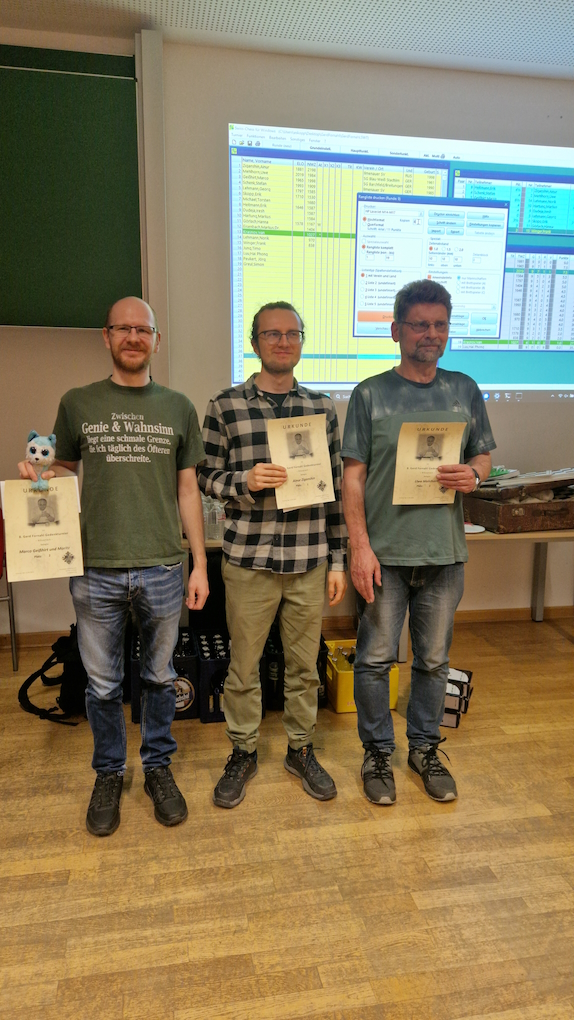
\includegraphics[width=\linewidth]{2024_04_Gerd_Fornahl_Gedenkturnier_8_03}
    \captionof{figure}{Siegerehrung Bild 3}
    \label{fig:gerd_fornahl_3}
\end{center}

\subsection{Siegerehrung Bild 4}
\begin{center}
    \includegraphics[width=\linewidth]{2024_04_Gerd_Fornahl_Gedenkturnier_8_04}
    \captionof{figure}{Siegerehrung Bild 4}
    \label{fig:gerd_fornahl_4}
\end{center}


\end{document}
